%This is a experiment example of ZhengXiaoyang's experiment report template

\documentclass[UTF8]{ctexart}
 
\usepackage{amsmath}
\usepackage{cases}
\usepackage{cite}
\usepackage{ctex}
\usepackage{graphicx}
\usepackage[margin=1in]{geometry}
\geometry{a4paper}
\usepackage{fancyhdr}
\pagestyle{fancy}
\fancyhf{}

\graphicspath{{picture/}}


\title{RLC稳态电路实验预习报告}
\graphicspath{{picture/}}


\title{RLC稳态电路实验预习报告}
\author{郑晓旸}
\date{\today}
\pagenumbering{arabic}

\begin{document}
%这里是文件的开头
\fancyhead[L]{郑晓旸}
\fancyhead[C]{RLC稳态}
\fancyfoot[C]{\thepage}

\maketitle
\tableofcontents
\newpage

\section{实验目的}
    \begin{enumerate}
            \item 了解电感和电容的电学特性 
            \item 深入理解 RLC 串联谐振电路的特性
            \item 掌握用示波器观察和测量稳态信号的方法
    \end{enumerate} 


\section{实验仪器}
\begin{enumerate}
    \item 数字示波器
    \item 信号发生器
    \item 九孔电路实验板
    \item 电学元件(电阻、电容、电感、导线等)
    \item 数字多用表
\end{enumerate}
\section{实验原理}

\subsection{电感器和电容器}

电感器和电容器是常见的无源电路元件。理想电感器的伏安特性为:
\begin{equation}
u(t) = L\frac{di(t)}{dt}
\end{equation}
其中,$u(t)$为电感两端电压,$i(t)$为通过电感的电流,$L$为电感值,单位为亨利(H)。

理想电容器的伏安特性为:
\begin{equation}
i(t) = C\frac{du(t)}{dt}
\end{equation}
其中,$i(t)$为流经电容的电流,$u(t)$为电容两端电压,$C$为电容值,单位为法拉(F)。

\subsection{RLC串联谐振电路}

如图\ref{fig:rlc_circuit}所示,RLC串联谐振电路由电阻$R$、电感$L$和电容$C$串联而成,交流电压源为$u(t)=u_0\sin(\omega t)$。
\begin{figure}[htbp]
\centering
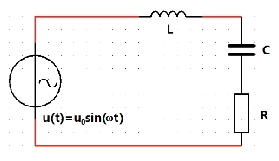
\includegraphics[width=0.6\textwidth]{rlc_circuit.png}
\caption{RLC串联谐振电路}\label{fig:rlc_circuit}
\end{figure}

根据基尔霍夫电压定律,电路方程为:
\begin{equation}
L\frac{d^2u_C(t)}{dt^2} + R\frac{du_C(t)}{dt} + \frac{1}{C}u_C(t) = u_0\sin(\omega t)
\end{equation}
其中,$u_C(t)$为电容两端电压。引入固有频率$\omega_0$和品质因数$Q$:
\begin{equation}
\omega_0 = \frac{1}{\sqrt{LC}}, \quad Q = \frac{1}{R}\sqrt{\frac{L}{C}}
\end{equation}
电路方程可改写为:
\begin{equation}
\frac{1}{\omega_0^2}\frac{d^2u_C(t)}{dt^2} + \frac{1}{Q\omega_0}\frac{du_C(t)}{dt} + u_C(t) = u_0\sin(\omega t)
\end{equation}

该方程的稳态解为:
\begin{equation}
\begin{cases}
\frac{u_C(t)}{u_0} = -\frac{Q\omega_0}{\omega}A\cos(\omega t + \phi) \\
\frac{u_R(t)}{u_0} = A\sin(\omega t + \phi) \\
\frac{u_L(t)}{u_0} = \frac{Q\omega}{\omega_0}A\cos(\omega t + \phi)
\end{cases}
\end{equation}
其中,
\begin{equation}
A = \frac{1}{\sqrt{1 + Q^2(\frac{\omega_0}{\omega} - \frac{\omega}{\omega_0})^2}}, \quad
\phi = \arctan\left[Q\left(\frac{\omega_0}{\omega} - \frac{\omega}{\omega_0}\right)\right]
\end{equation}

$A(\omega)$和$\phi(\omega)$分别称为电路的幅频特性和相频特性,统称为频率特性。当$\omega=\omega_0$时,电路达到谐振状态,此时$A(\omega_0)=1$,$\phi(\omega_0)=0$。品质因数$Q$反映了谐振时的电压放大倍数、频率选择性以及能量耗散的快慢。

\section{实验方法}

本实验采用示波器和信号发生器测量RLC串联谐振电路的特性,实验电路如图\ref{fig:measure_circuit}所示。

\subsection{谐振频率测量}

\begin{figure}[htbp]
\centering
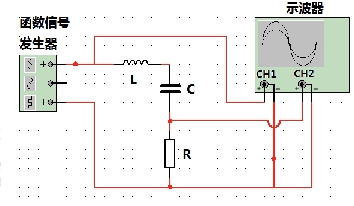
\includegraphics[width=0.4\textwidth]{measure_circuit.png}
\caption{谐振频率测量电路}\label{fig:measure_circuit}
\end{figure}

将信号发生器的输出和电阻两端电压分别接入示波器的两个通道,调节信号发生器频率,直到两个信号同相位,此时输入信号频率即为谐振频率$\omega_0$。示波器可使用XY模式方便判断两信号是否同相位,如图\ref{fig:xy_mode}所示。

\begin{figure}[htbp]
\centering
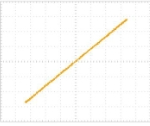
\includegraphics[width=0.4\textwidth]{xy_mode.png}
\caption{示波器XY模式显示两个同频率正弦信号}\label{fig:xy_mode}
\end{figure}

\subsection{品质因数测量}

达到谐振状态后,测量电容两端电压幅值$U_C$和输入信号幅值$U_0$,品质因数$Q$为:
\begin{equation}
Q = \frac{U_C}{U_0}
\end{equation}

示波器可使用光标手动测量或自动测量电压幅值。注意调节垂直灵敏度,使信号尽量放大但不超出屏幕范围,以减小读数误差。

实际电感存在等效电阻$R_L$,计算品质因数的理论值时,应使用等效电阻$R_{eq}=R+R_L$代替电路中的电阻$R$。$R_L$可用LCR测试仪在谐振频率下测得。

此外,也可根据相频特性曲线$\phi(\omega)$在$\omega_0$处的变化率计算品质因数:
\begin{equation}
Q = -\frac{\omega_0}{2}\left.\frac{d\phi(\omega)}{d\omega}\right|_{\omega=\omega_0}
\end{equation}

\subsection{频率特性测量}

保持图\ref{fig:measure_circuit}的测量电路,改变信号发生器频率,在每个频率点测量$U_R$和$U_0$的幅值比$A=U_R/U_0$以及两信号的相位差$\phi$。为与理论值比较,需将幅值比修正为:
\begin{equation}
A' = \frac{R+R_L}{R}A
\end{equation}

相位差可用示波器光标测量,将两信号调至屏幕水平中线,测出它们的周期$T$和同相位点的时间差$\delta T$(超前为正,滞后为负),则相位差为:
\begin{equation}
\phi = \frac{\delta T}{T} \times 360^\circ
\end{equation}

频率选取应覆盖低频到高频,且相位差变化范围不小于$160^\circ$。每隔$5^\circ$左右选取一个频率点,获得幅频和相频特性曲线。

\section{预习思考题}

\begin{enumerate}
    \item \textbf{保持$L$和$C$不变,增大$R$,电路的谐振频率与品质因数如何改变?}
    
    根据RLC串联谐振电路的理论分析,固有频率$\omega_0$和品质因数$Q$的表达式为:
    \begin{equation}
    \omega_0 = \frac{1}{\sqrt{LC}}, \quad Q = \frac{1}{R}\sqrt{\frac{L}{C}}
    \end{equation}
    \begin{enumerate}
    \item 当保持电感$L$和电容$C$不变,增大电阻$R$时:

    谐振频率$\omega_0$:
    \begin{equation}
    \omega_0 = \frac{1}{\sqrt{LC}}
    \end{equation}
    由于$L$和$C$保持不变,谐振频率$\omega_0$也不会改变。

    \item 品质因数$Q$:
    \begin{equation}
    Q = \frac{1}{R}\sqrt{\frac{L}{C}}
    \end{equation}
    当$R$增大时,品质因数$Q$与$R$成反比,因此$Q$将减小。
    \end{enumerate}
    品质因数$Q$的变化会影响电路的频率选择性和谐振峰的尖锐  程度。$Q$值越大,频率选择性越好,谐振峰越尖锐;$Q$值越小,频率选择性越差,谐振峰越平坦。

    综上所述,保持$L$和$C$不变,增大$R$时:
    \begin{itemize}
    \item 谐振频率$\omega_0$保持不变;
    \item 品质因数$Q$减小,频率选择性变差,谐振峰变平坦。
    \end{itemize}
    
    \item \textbf{对于RLC串联谐振的频率响应曲线,当频率取对数坐标时,证明幅频特性曲线关于$\omega=\omega_0$是对称的,而相频特性曲线是反对称的.}
    
    对于RLC串联谐振电路的频率响应曲线,当频率取对数坐标时,幅频特性曲线$A(\omega)$和相频特性曲线$\phi(\omega)$分别满足以下关系:

\begin{equation}
A(\omega) = \frac{1}{\sqrt{1 + Q^2(\frac{\omega_0}{\omega} - \frac{\omega}{\omega_0})^2}}
\end{equation}

\begin{equation}
\phi(\omega) = \arctan\left[Q\left(\frac{\omega_0}{\omega} - \frac{\omega}{\omega_0}\right)\right]
\end{equation}

当频率取对数坐标时,令$x=\log(\omega/\omega_0)$,则$\omega=\omega_0e^x$。将其代入$A(\omega)$和$\phi(\omega)$的表达式,得到:

\begin{equation}
A(x) = \frac{1}{\sqrt{1 + Q^2(e^{-x} - e^x)^2}}
\end{equation}

\begin{equation}
\phi(x) = \arctan\left[Q\left(e^{-x} - e^x\right)\right]
\end{equation}

对于幅频特性曲线$A(x)$,有:
\begin{equation}
A(-x) = \frac{1}{\sqrt{1 + Q^2(e^x - e^{-x})^2}} = \frac{1}{\sqrt{1 + Q^2(e^{-x} - e^x)^2}} = A(x)
\end{equation}
因此,$A(x)$关于$x=0$(即$\omega=\omega_0$)对称。

对于相频特性曲线$\phi(x)$,有:
\begin{equation}
\phi(-x) = \arctan\left[Q\left(e^x - e^{-x}\right)\right] = \arctan\left[-Q\left(e^{-x} - e^x\right)\right] = -\phi(x)
\end{equation}
因此,$\phi(x)$关于$x=0$(即$\omega=\omega_0$)反对称。
    
    \item \textbf{如果$Q\gg1$,如何理解谐振时电容上的电压远高于电路的输入电压?}
    
    在谐振状态下,电容两端电压为:
\begin{equation}
u_C(t) = -Q u_0 \cos(\omega_0 t)
\end{equation}

电容两端电压幅值为输入电压幅值的$Q$倍。当$Q\gg1$时,电容两端电压可远高于输入电压。这可以从能量的角度理解:

在谐振过程中,电感和电容不断交换能量。设电路在$t=0$时的初始能量为$E_0$,则在谐振过程中,电路总能量保持不变:
\begin{equation}
E = \frac{1}{2}C u_C^2(t) + \frac{1}{2}L i^2(t) = E_0
\end{equation}

由于$i(t)=C\frac{du_C(t)}{dt}$,代入上式得:
\begin{equation}
E = \frac{1}{2}C u_C^2(t) + \frac{1}{2}LC^2 \left(\frac{du_C(t)}{dt}\right)^2 = E_0
\end{equation}

在谐振状态下,$u_C(t)$和$\frac{du_C(t)}{dt}$的幅值分别为$QU_0$和$\omega_0 QU_0$,代入上式得:
\begin{equation}
E_0 = \frac{1}{2}C(QU_0)^2 + \frac{1}{2}LC^2(\omega_0 QU_0)^2 = \frac{1}{2}C(QU_0)^2 + \frac{1}{2}C(QU_0)^2 = C(QU_0)^2
\end{equation}

可见,谐振时电路总能量为$C(QU_0)^2$,是输入能量$\frac{1}{2}CU_0^2$的$4Q^2$倍。这表明,在谐振过程中,电感和电容不断交换能量,使得能量逐渐累积,当$Q\gg1$时,电路内能量可远大于输入能量,因此电容两端电压也远高于输入电压。
    
    \item \textbf{在谐振状态,能否用电感器上的电压与输入电压的幅度比计算品质因数?}
    
    在谐振状态下,不能直接用电感两端电压与输入电压的幅值比计算品质因数。下面给出具体推导说明:

在谐振频率$\omega_0$下,电感两端电压为:
\begin{equation}
u_L(t) = \frac{Q\omega_0}{\omega_0}u_0\cos(\omega_0 t) = Qu_0\cos(\omega_0 t)
\end{equation}

电感两端电压幅值$U_L$与输入电压幅值$U_0$之比为:
\begin{equation}
\frac{U_L}{U_0} = Q
\end{equation}

但是,这个比值虽然在数值上等于品质因数$Q$,却不能直接用于计算$Q$。因为在谐振状态下,电感两端电压与输入电压同相位,而品质因数的定义是电容两端电压与输入电压幅值之比:
\begin{equation}
Q = \frac{U_C}{U_0}
\end{equation}

其中,电容两端电压为:
\begin{equation}
u_C(t) = -Qu_0\cos(\omega_0 t)
\end{equation}

电容两端电压与输入电压反相,幅值是输入电压的$Q$倍。因此,在谐振状态下,只能用电容两端电压与输入电压的幅值比来计算品质因数,而不能用电感两端电压。
    
    \item \textbf{实验中能否根据电阻上的电压达到最大值判断电路达到谐振?}
    
    不能根据电阻两端电压达到最大值判断电路达到谐振。下面给出详细推导:

根据电路的频率特性,电阻两端电压为:
\begin{equation}
u_R(t) = u_0 A \sin(\omega t + \phi)
\end{equation}
其中,幅值$A$和相位差$\phi$分别为:
\begin{equation}
A = \frac{1}{\sqrt{1 + Q^2(\frac{\omega_0}{\omega} - \frac{\omega}{\omega_0})^2}}, \quad
\phi = \arctan\left[Q\left(\frac{\omega_0}{\omega} - \frac{\omega}{\omega_0}\right)\right]
\end{equation}

要找到$u_R(t)$幅值最大时对应的频率,需对$A$求导并令其为零:
\begin{equation}
\frac{dA}{d\omega} = \frac{Q^2(\frac{\omega_0}{\omega^2} + \frac{1}{\omega_0})}{[1 + Q^2(\frac{\omega_0}{\omega} - \frac{\omega}{\omega_0})^2]^{3/2}} = 0
\end{equation}

解得:
\begin{equation}
\omega_{max} = \omega_0\sqrt{1 + \frac{1}{2Q^2}}
\end{equation}

可见,$u_R(t)$幅值最大时对应的频率$\omega_{max}$与谐振频率$\omega_0$并不完全相等,而是略大于$\omega_0$。当$Q \gg 1$时,两者较为接近:
\begin{equation}
\omega_{max} \approx \omega_0(1 + \frac{1}{4Q^2})
\end{equation}

但在$Q$较小时,误差会比较显著。因此,不能根据电阻两端电压达到最大值来判断电路达到谐振。准确的判断方法应该是观察输入信号与电阻两端电压的相位差,当相位差为零时,电路达到谐振。
    
    \item \textbf{对于相-频特性曲线$\phi(\omega)$,除了可根据$\phi(\omega)=\pm\frac{\pi}{4}$确定带宽,从而计算品质因数,还可以根据$\phi(\omega)$在$\omega_0$处的变化率测量品质因数。证明
    \begin{equation*}
        -\omega_0\phi'(\omega_0)=2Q
    \end{equation*}
    根据上面性质,如何测量电路的品质因数?}
    
    对于相频特性曲线$\phi(\omega)$,由公式
\begin{equation}
\phi(\omega) = \arctan\left[Q\left(\frac{\omega_0}{\omega} - \frac{\omega}{\omega_0}\right)\right]
\end{equation}
求导可得:
\begin{align}
\phi'(\omega) &= \frac{Q}{\left[Q\left(\frac{\omega_0}{\omega} - \frac{\omega}{\omega_0}\right)\right]^2 + 1} \cdot \left(-\frac{\omega_0}{\omega^2} - \frac{1}{\omega_0}\right) \\
&= \frac{Q}{\left[Q\left(\frac{\omega_0}{\omega} - \frac{\omega}{\omega_0}\right)\right]^2 + 1} \cdot \left(-\frac{\omega_0^2 + \omega^2}{\omega^2\omega_0}\right)
\end{align}
当$\omega = \omega_0$时,
\begin{equation}
\phi'(\omega_0) = \frac{Q}{1} \cdot \left(-\frac{2\omega_0^2}{\omega_0^2\omega_0}\right) = -\frac{2Q}{\omega_0}
\end{equation}
即
\begin{equation}
-\omega_0\phi'(\omega_0) = 2Q
\end{equation}

根据上述性质,测量电路品质因数的步骤如下:
\begin{enumerate}
\item 测得谐振频率$\omega_0$;
\item 在$\omega_0$附近选取两个频率点$\omega_1$和$\omega_2$,测量相应的相位差$\phi_1$和$\phi_2$;
\item 计算$\omega_0$处的相位变化率:
\begin{equation}
\phi'(\omega_0) \approx \frac{\phi_2 - \phi_1}{\omega_2 - \omega_1}
\end{equation}
\item 代入公式计算品质因数:
\begin{equation}
Q \approx -\frac{\omega_0}{2} \cdot \frac{\phi_2 - \phi_1}{\omega_2 - \omega_1}
\end{equation}
\end{enumerate}
    
\end{enumerate}

\end{document}
